\section{Experiments}
\label{sec_exp}

We evaluate the proposed \textbf{MTL} and \textbf{HT meta-batch} in terms of few-shot recognition accuracy and model convergence speed.
%
Below we describe the datasets and detailed settings, followed by an ablation study and a comparison to state-of-the-art methods.

\subsection{Datasets and implementation details}
\label{sec_dataset}

We conduct few-shot learning experiments on two benchmarks, miniImageNet~\cite{VinyalsBLKW16} and Fewshot-CIFAR100 (FC100)~\cite{OreshkinNIPS18}. 
%
miniImageNet is widely used in related works~\cite{FinnAL17, RaviICLR2017, GrantICLR2018, FranceschiICML18, MunkhdalaiICML18}. FC100 is newly proposed in~\cite{OreshkinNIPS18} and is more challenging in terms of lower image resolution and stricter training-test splits than miniImageNet.

\myparagraph{miniImageNet} was proposed by Vinyals \emph{et al}.~\cite{VinyalsBLKW16} for few-shot learning evaluation. 
%
Its complexity is high due to the use of ImageNet images, but requires less resource and infrastructure than running on the full ImageNet dataset~\cite{Russakovsky2015}. 
%
In total, there are $100$ classes with $600$ samples of $84 \times 84$ color images per class.
%
These $100$ classes are divided into $64$, $16$, and $20$ classes respectively for sampling tasks for meta-training, meta-validation and meta-test, following related works~\cite{FinnAL17, RaviICLR2017, GrantICLR2018, FranceschiICML18, MunkhdalaiICML18}.


\myparagraph{Fewshot-CIFAR100 (FC100)}
is based on the popular object classification dataset CIFAR100 \cite{CIFAR100}. The splits were proposed by~\cite{OreshkinNIPS18} (Please check details in the supplementary).
%
It offers a more challenging scenario with lower image resolution and more challenging meta-training/test splits that are separated according to object super-classes.
%
It contains $100$ object classes and each class has $600$ samples of $32 \times 32$ color images.
%
%
The $100$ classes belong to $20$ super-classes. Meta-training data are from $60$ classes belonging to $12$ super-classes. Meta-validation and meta-test sets contain $20$ classes belonging to $4$ super-classes, respectively. 
These splits accord to super-classes, thus minimize the information overlap between training and val/test tasks. 

%%%%%%%%%%%%%%%%%%%%%% shared settings as follows,
The following settings are used on both datasets.
We train a large-scale DNN with all training datapoints (Section~\ref{sec_large_scale_pretrain}) and stop this training after $10k$ iterations.
%
We use the same task sampling method as related works~\cite{FinnAL17, RaviICLR2017}. Specifically, 1) we consider the 5-class classification and 2) we sample 5-class, 1-shot (5-shot or 10-shot) episodes to contain 1 (5 or 10) samples for train episode, and $15$ (uniform) samples for episode test.
Note that in the state-of-the-art work~\cite{OreshkinNIPS18}, $32$ and $64$ samples are respectively used in 5-shot and 10-shot settings for episode test.
%
In total, we sample $8k$ tasks for meta-training (same for w/ and w/o HT meta-batch), and respectively sample $600$ random tasks for meta-validation and meta-test. 
Please check the supplementary document (or \href{https://github.com/y2l/meta-transfer-learning-tensorflow}{GitHub repository}) for other implementation details, e.g. learning rate and dropout rate.


\myparagraph{Network architecture.} 
We present the details for
the Feature Extractor $\Theta$, 
MTL meta-learner with \emph{Scaling} $\Phi_{S_1}$ and \emph{Shifting} $\Phi_{S_2}$, 
and MTL base-learner (classifier) $\theta$. 

\myparagraph{The architecture of $\Theta$} have two options, ResNet-12 and 4CONV, commonly used in related works~\cite{FinnAL17, VinyalsBLKW16, RaviICLR2017, MunkhdalaiICML18, MishraICLR2018, OreshkinNIPS18}.
%
\myparagraph{4CONV} consists of $4$ layers with $3\times 3$ convolutions and $32$ filters, followed by batch normalization (BN)~\cite{IoffeICML15}, a ReLU nonlinearity, and $2\times 2$ max-pooling.
%
\myparagraph{ResNet-12} is more popular in recent works~\cite{OreshkinNIPS18, MishraICLR2018, FranceschiICML18, MunkhdalaiICML18}. It contains $4$ residual blocks and each block has $3$ CONV layers with $3\times 3$ kernels.
%
At the end of each residual block, a $2\times 2$ max-pooling layer is applied. The number of filters starts from $64$ and is doubled every next block. 
%
Following $4$ blocks, there is a mean-pooling layer to compress the output feature maps to a feature embedding.
\myparagraph{The difference} between using 4CONV and using ResNet-12 in our methods is that ResNet-12 MTL sees the large-scale data training, but 4CONV MTL is learned from scratch because of its poor performance for large-scale data training (see results in the supplementary).
%
Therefore, we emphasize the experiments of using ResNet-12 MTL for its superior performance.
%
\myparagraph{The architectures of $\Phi_{S_1}$ and $\Phi_{S_2}$} are generated according to the architecture of $\Theta$, as introduced in Section~\ref{sec_meta_transfer}. That is when using ResNet-12 in MTL, $\Phi_{S_1}$ and $\Phi_{S_2}$ also have 12 layers, respectively.
%%
%
\myparagraph{The architecture of $\theta$} is an FC layer. We empirically find that a single FC layer is faster to train and more effective for classification than multiple layers.
(see comparisons in the supplementary).


\begin{figure*}
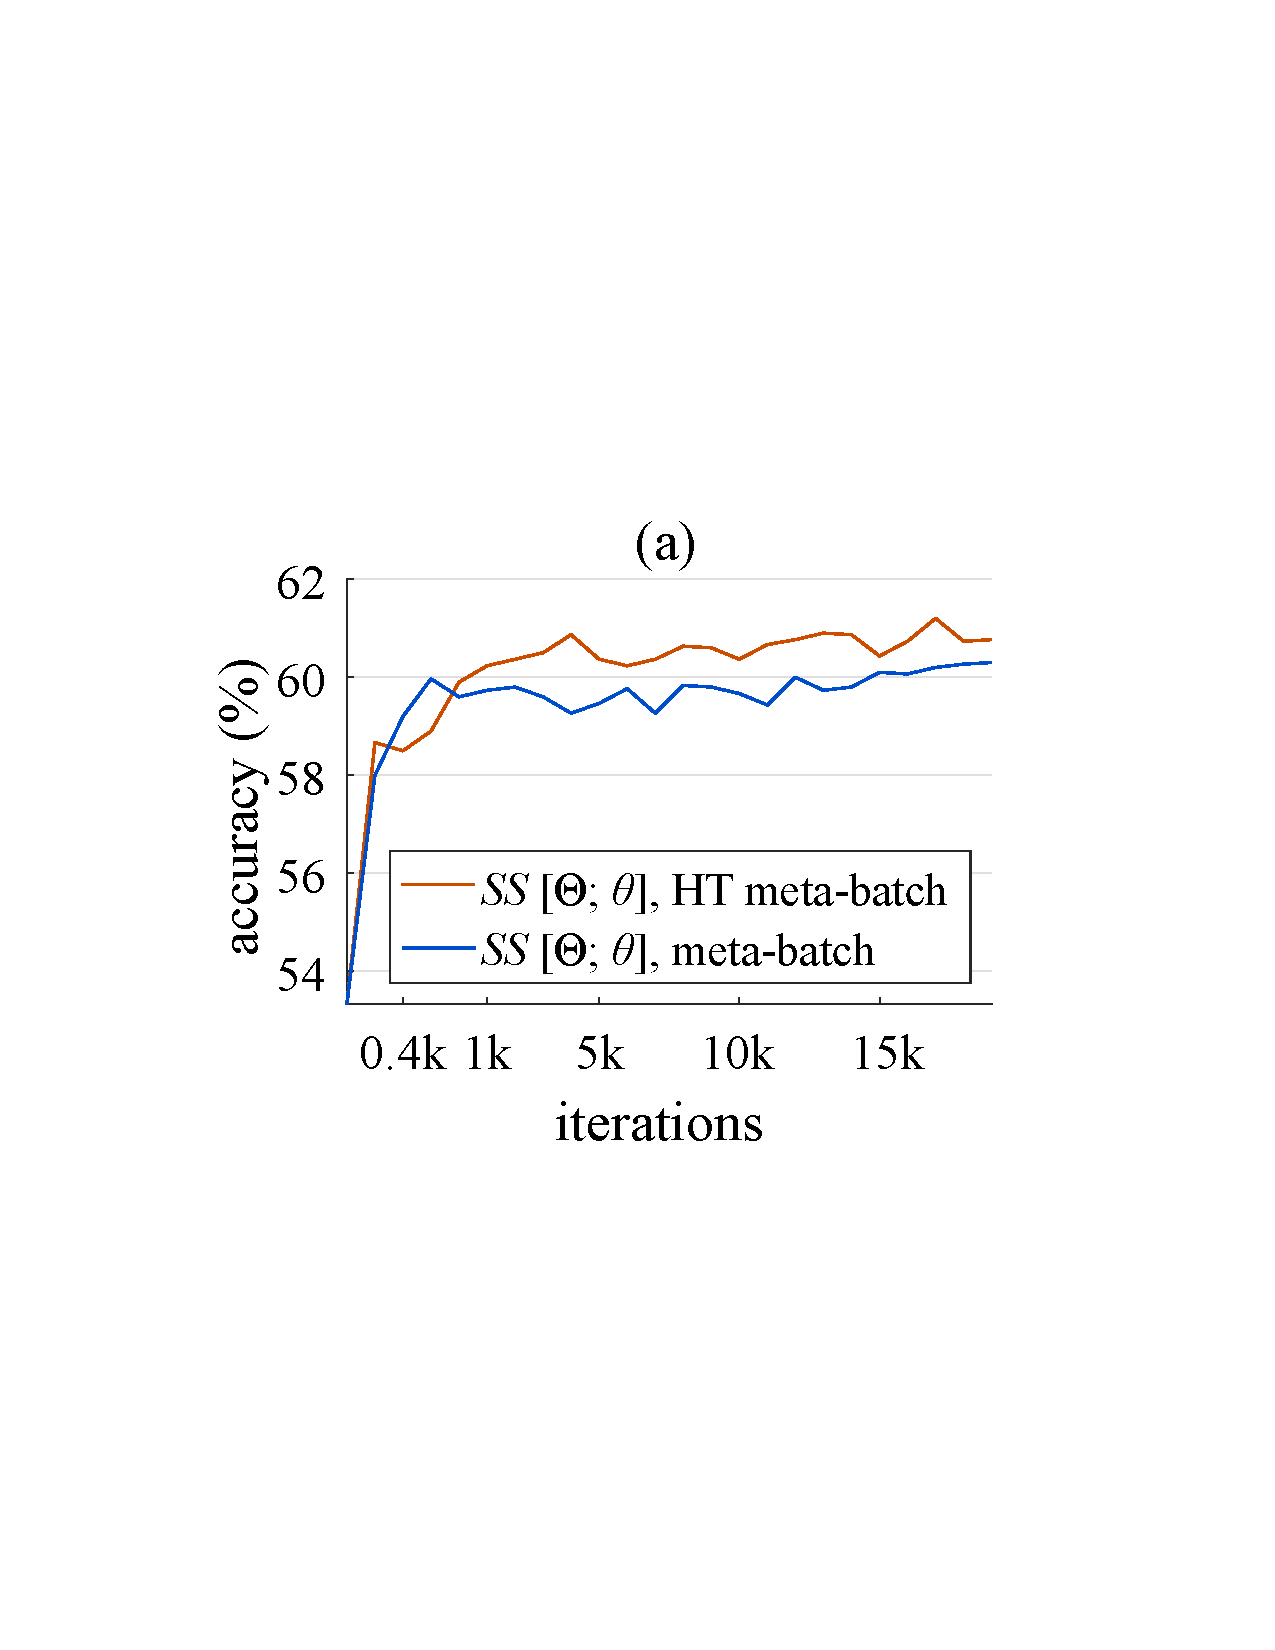
\includegraphics[height=1.09in]{mini1shot.pdf}
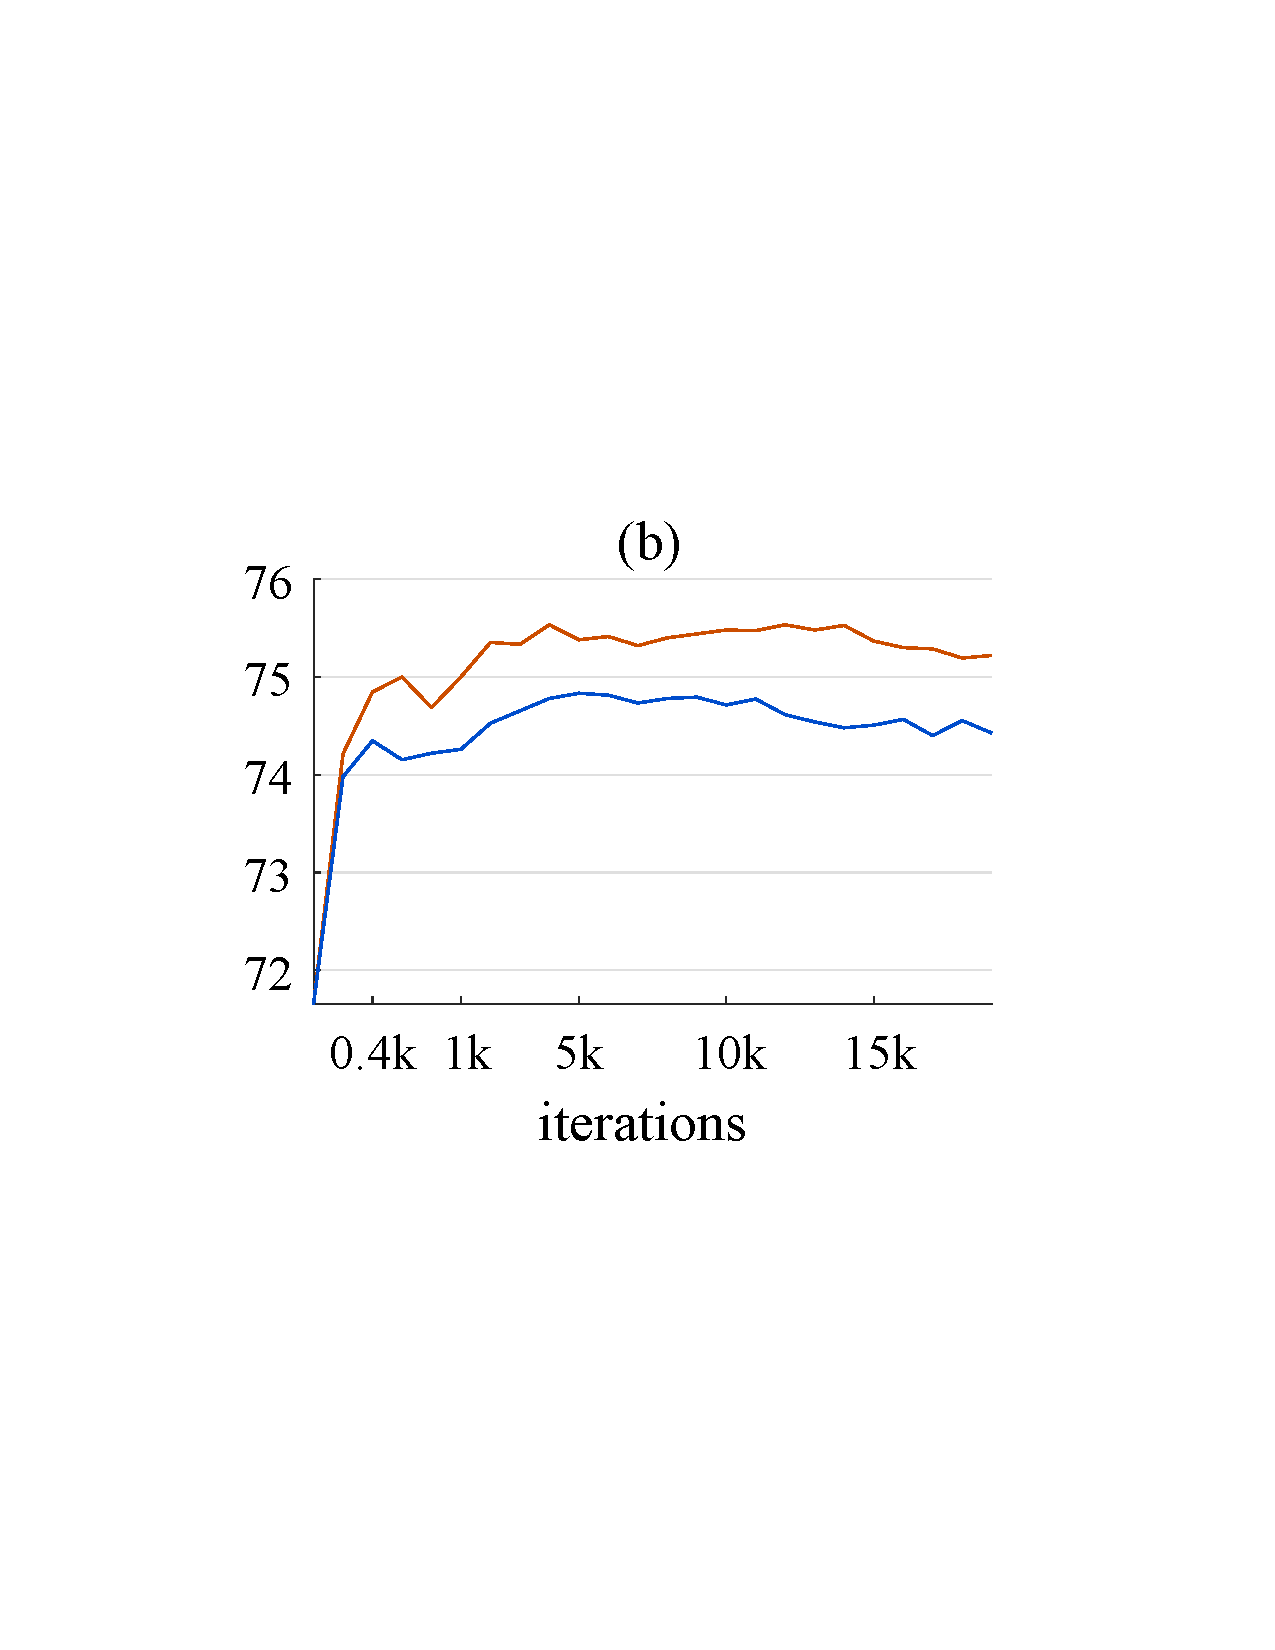
\includegraphics[height=1.09in]{mini5shot.pdf}
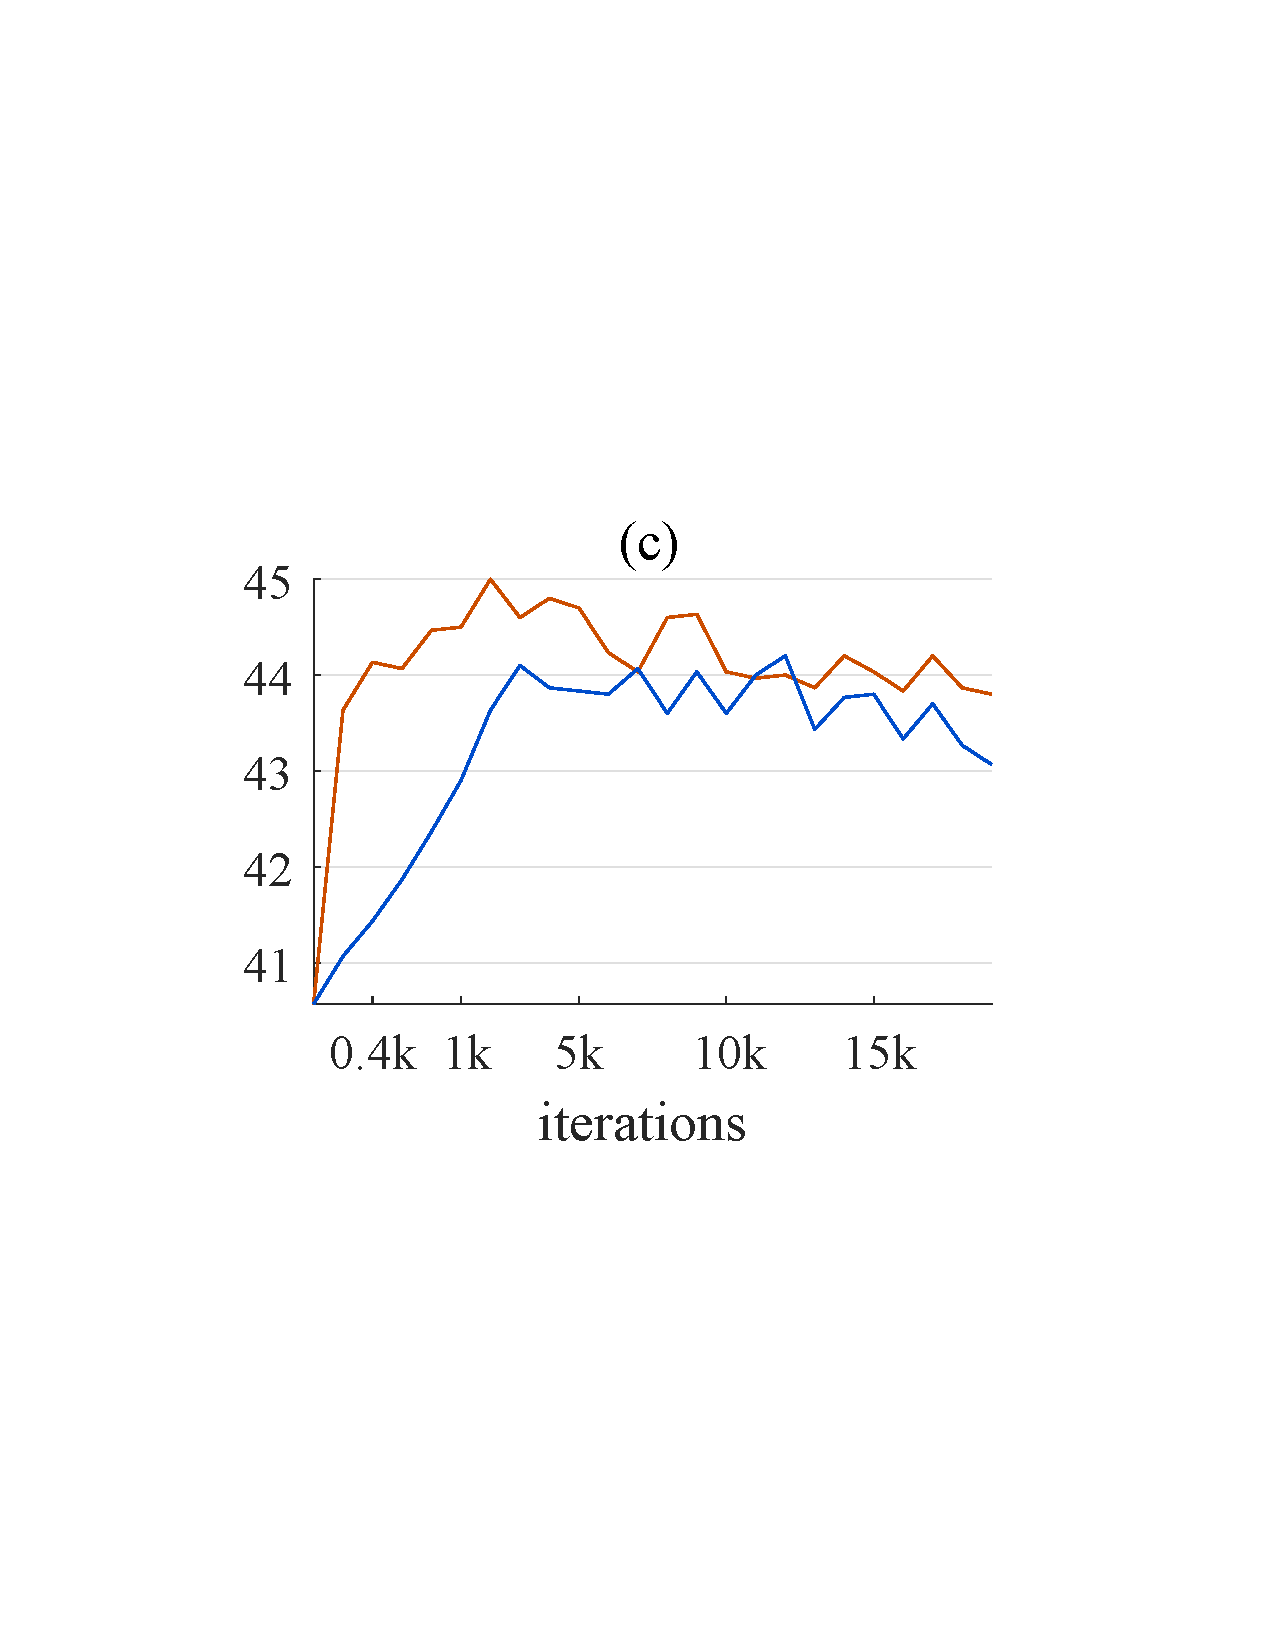
\includegraphics[height=1.09in]{fc1shot.pdf}
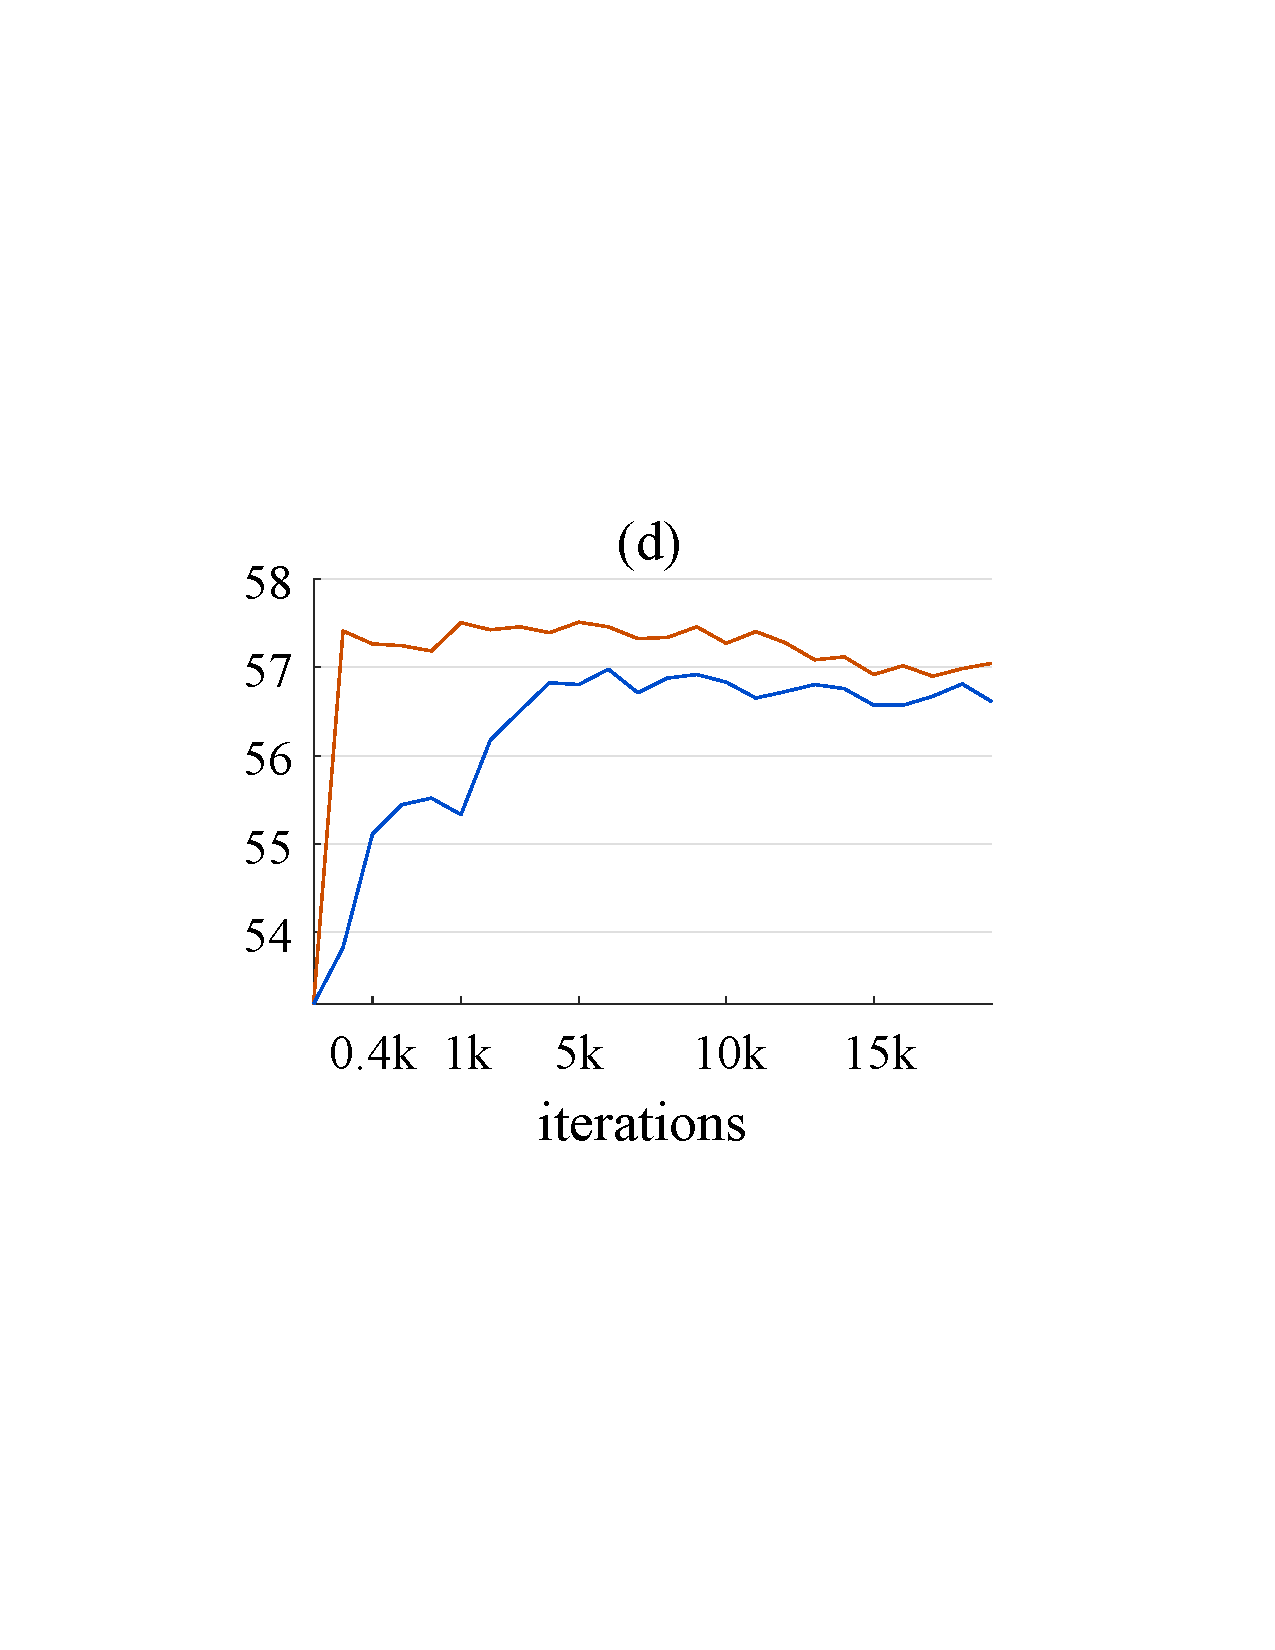
\includegraphics[height=1.09in]{fc5shot.pdf}
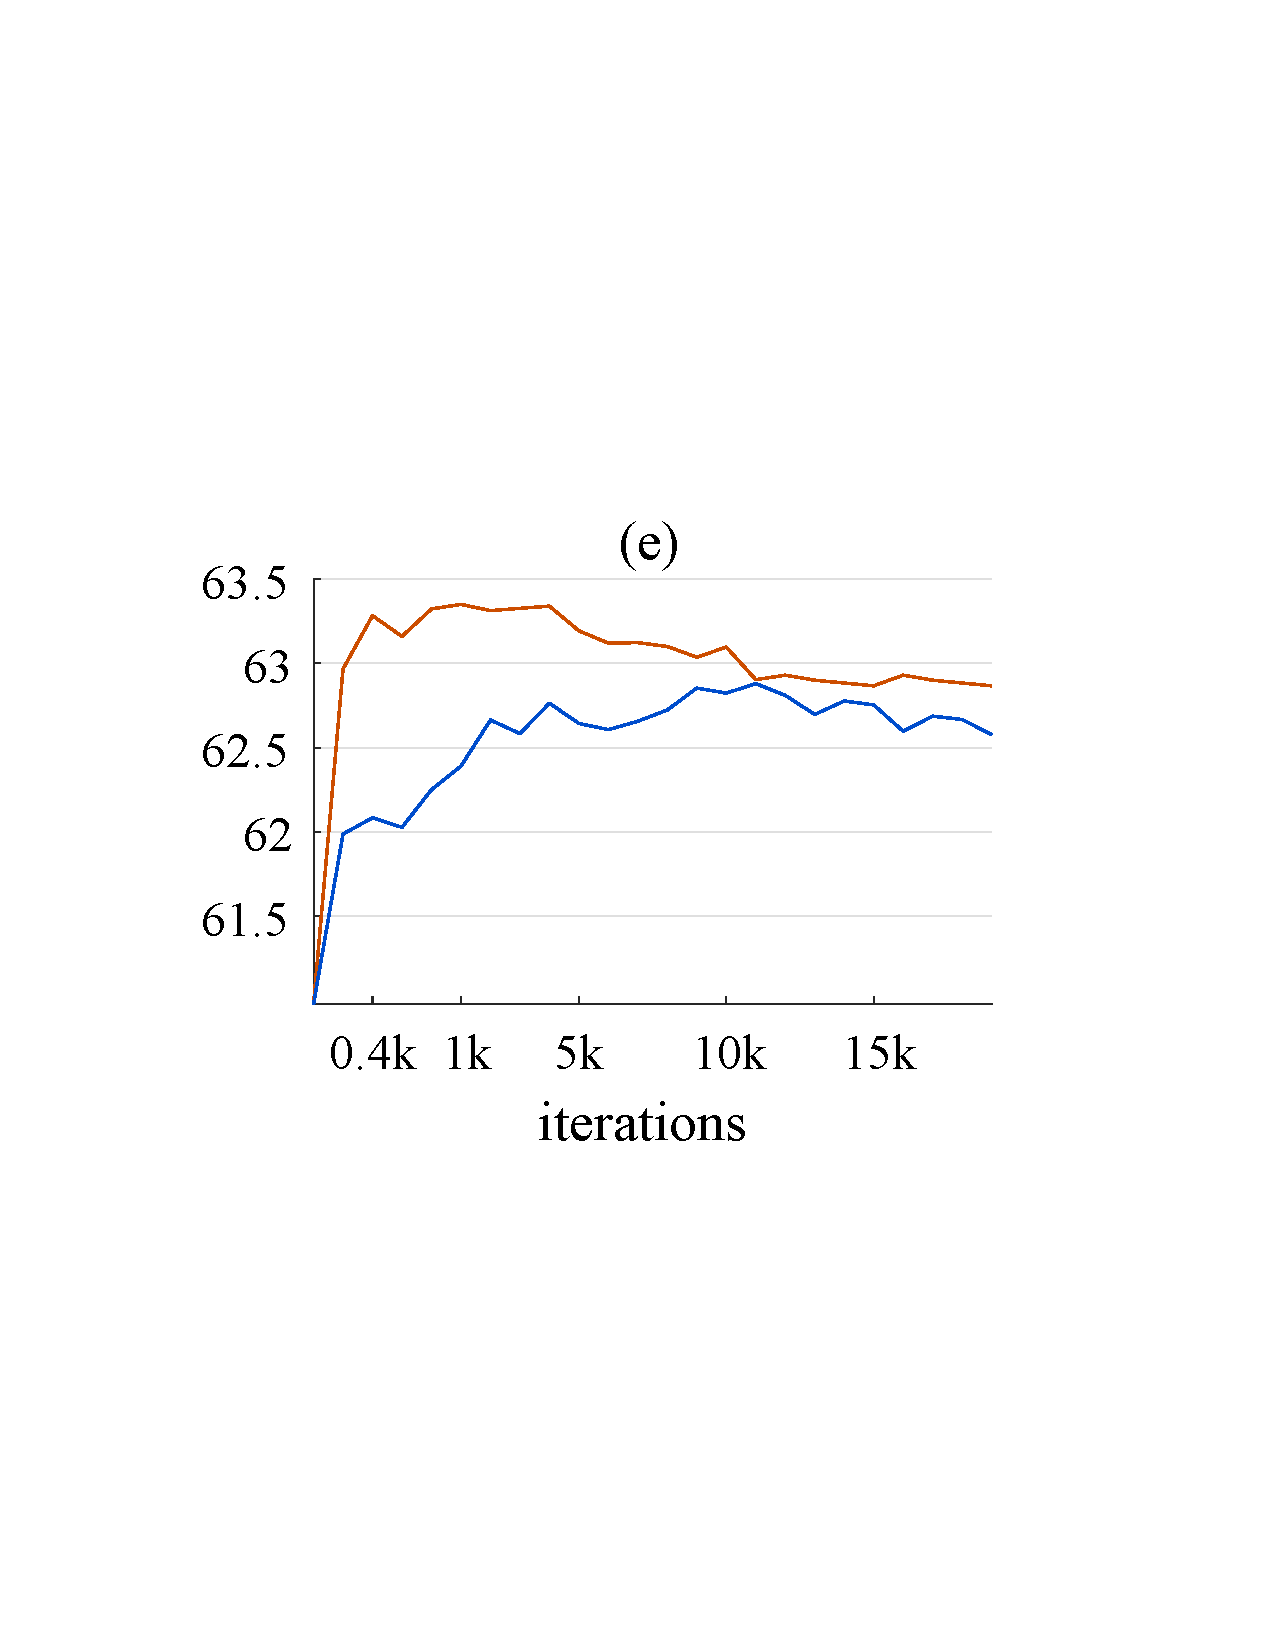
\includegraphics[height=1.09in]{fc10shot.pdf}
\caption{(a)(b) show the results of 1-shot and 5-shot on miniImageNet; (c)(d)(e) show the results of 1-shot, 5-shot and 10-shot on FC100.}
\vspace{-0.3cm}
\label{fig_mini_fc100}
\end{figure*}

\subsection{Ablation study setting}
\label{sec_setting}

In order to show the effectiveness of our approach, we design some ablative settings: 
%
two baselines without meta-learning but more classic learning,
three baselines of \emph{Fine-Tuning} (\emph{FT}) on smaller number of parameters (Table~\ref{tab_ablation_study}), and
%
two MAML variants using our deeper pre-trained model and HT meta-batch (Table~\ref{table_mini} and Table~\ref{table_fc100}).
Note that the alternative meta-learning operation to \emph{SS} is the \emph{FT} used in MAML.
Some bullet names are explained as follows.

\myparagraph{\emph{update} $[\Theta; \theta]$ (or $\theta$).} 
There is no meta-training phase. During test phase, each task has its whole model $[\Theta; \theta]$ (or the classifier $\theta$) updated on $\mathcal{T}^{(tr)}$, and then tested on $\mathcal{T}^{(te)}$.

\myparagraph{\emph{FT} $[\Theta 4; \theta]$ (or $\theta$).}
These are straight-forward ways to define a smaller set of meta-learner parameters than MAML.
We can freeze low-level pre-trained layers and meta-learn the classifier layer $\theta$ with (or without) high-level CONV layer $\Theta 4$ that is the 4th residual block of ResNet-12.


\subsection{Results and analysis}
\label{sec_result}

\begin{table}[b]
\centering
\vspace{-0.4cm}
\small
\begin{tabular*}{8cm}
{lcccccc}
\toprule 
& \multicolumn{2}{c}{miniImageNet} & & \multicolumn{3}{c}{FC100} \\
\cmidrule{2-3}\cmidrule{5-7}
& 1 (shot) & 5 & & 1 & 5 & 10 \\
\midrule[1pt]
\emph{update} $[\Theta; \theta]$ & 45.3 & 64.6  & & 38.4 & 52.6 & 58.6 \\
\emph{update} $\theta$ & 50.0 & 66.7  & & 39.3 & 51.8 & 61.0 \\
\midrule[1pt]	
% \midrule[1pt]
\emph{FT} $\theta$  & 55.9 & 71.4  & & 41.6 & 54.9 & 61.1 \\
\emph{FT} $[\Theta4; \theta]$ & 57.2 & 71.6 & & 40.9 & 54.3 & 61.3 \\
% \emph{FT} $[\Theta3,\Theta4; \theta]$ & 58.1 & 70.9 & & 41.5 & 53.7 & 61.3 \\
\emph{FT} $[\Theta; \theta]$  & 58.3 & 71.6  & & 41.6 & 54.4 & 61.2 \\
\midrule[1pt]
\emph{SS} $[\Theta4; \theta]$ & 59.2 & 73.1  & &42.4 &55.1 &61.6 \\
% \emph{SS} $[\Theta3,\Theta4; \theta]$ & 59.4 & 73.4 & &42.5 &54.5 & 61.7\\
% \midrule[1pt]
\emph{SS $[\Theta; \theta]$}\textbf{(Ours)} & 60.2 & 74.3 & & 43.6 & 55.4 & 62.4  \\
\bottomrule[1pt]
\end{tabular*}
\vspace{0.1cm}
\caption{Classification accuracy (\%) using ablative models, on two datasets. ``meta-batch'' and ``ResNet-12(pre)'' are used.}
\label{tab_ablation_study}
\end{table}

\begin{table*}
%   \vspace{0.2cm}
  \small
  \centering
  \begin{tabular}{l l lcc}
    \toprule
     \multicolumn{2}{c}{Few-shot learning method} & Feature extractor & 1-shot & 5-shot \\
    \midrule
    \multirow{2}{*}{\emph{Data augmentation}}
    & Adv. ResNet, \cite{Mehrotra2017} & WRN-40 (pre) & 55.2 & 69.6 \\
    & Delta-encoder, \cite{SchwartzNIPS18} & VGG-16 (pre) & 58.7 & 73.6 \\
    \midrule  
    \multirow{3}{*}{\emph{Metric learning}}
    &Matching Nets, \cite{VinyalsBLKW16} & 4 CONV & 43.44 $\pm$ $0.77$ & 55.31 $\pm$  $0.73$ \\
    &ProtoNets, \cite{SnellSZ17} & 4 CONV & 49.42 $\pm$ $0.78$ & 68.20 $\pm$ $0.66$\\
    &CompareNets, \cite{SungCVPR2018} & 4 CONV & 50.44 $\pm$ $0.82$ & 65.32 $\pm$ $0.70$\\
         \midrule
    \multirow{3}{*}{\emph{Memory network}} 
    & Meta Networks, \cite{MunkhdalaiICML2017} & 5 CONV  & 49.21 $\pm$ $0.96$ & -- \\
    & SNAIL, \cite{MishraICLR2018} & ResNet-12 (pre)${}^{\diamond}$  & 55.71 $\pm$ $0.99$  & 68.88 $\pm$ $0.92$\\
    & TADAM, \cite{OreshkinNIPS18} & ResNet-12 (pre)${}^{\dag}$  & 58.5 $\pm$ $0.3$  & \textbf{76.7} $\mathbf{\pm}$ $\mathbf{0.3}$\\
    \midrule
    \multirow{6}{*}{\emph{Gradient descent}}
    & MAML, \cite{FinnAL17} & 4 CONV & 48.70 $\pm$ $1.75$ & 63.11 $\pm$ $0.92$ \\
    & Meta-LSTM, \cite{RaviICLR2017} & 4 CONV & 43.56 $\pm$ $0.84$ & 60.60 $\pm$ $0.71$ \\
    & Hierarchical Bayes, \cite{GrantICLR2018} & 4 CONV  & 49.40 $\pm$ $1.83$ & -- \\
    & Bilevel Programming, \cite{FranceschiICML18} & ResNet-12${}^{\diamond}$   & 50.54 $\pm$ $0.85$  & 64.53 $\pm$ $0.68$\\
    & MetaGAN, \cite{ZhangNIPS2018MetaGAN} & ResNet-12 & 52.71 $\pm$ $0.64$  & 68.63 $\pm$ $0.67$ \\
    & adaResNet, \cite{MunkhdalaiICML18} & ResNet-12${}^{\ddag}$   & 56.88 $\pm$ $0.62$ & 71.94 $\pm$ $0.57$ \\
    \midrule
    MAML, HT  & \emph{FT} $[\Theta; \theta]$, HT meta-batch & 4 CONV & 49.1 $\pm$ $1.9$ & 64.1 $\pm$ $0.9$ \\
    MAML deep, HT  & \emph{FT} $[\Theta; \theta]$, HT meta-batch & ResNet-12 (pre) & 59.1 $\pm$ $1.9$ & 73.1 $\pm$ $0.9$ \\
    \midrule
    \multirow{2}{*}{\textbf{MTL (Ours)}}
     & \emph{SS} $[\Theta; \theta]$, meta-batch & ResNet-12 (pre) & 60.2 $\pm$ $1.8$ & 74.3 $\pm$ $0.9$\\
     & \emph{SS} $[\Theta; \theta]$, HT meta-batch & ResNet-12 (pre) & \textbf{61.2} $\mathbf{\pm}$ $\mathbf{1.8}$ & \textbf{75.5} $\mathbf{\pm}$ $\mathbf{0.8}$\\
  \bottomrule
    \multicolumn{5}{l}{${}^{\diamond}$Additional 2 convolutional layers { } ${}^{\ddag}$Additional 1 convolutional layer { } ${}^{\dag}$Additional 72 fully connected layers}\\
\end{tabular}
  \vspace{0.2cm}
  \caption{The 5-way, 1-shot and 5-shot classification accuracy ($\%$) on miniImageNet dataset. ``pre'' means pre-trained for a single classification task using all training datapoints.}
    \label{table_mini}
\end{table*}


\begin{table*}[t]
  \small
  \centering
  \begin{tabular}{l l lccc}
    \toprule
     \multicolumn{2}{c}{Few-shot learning method} & Feature extractor & 1-shot & 5-shot & 10-shot \\
    \midrule    
    \multirow{1}{*}{\emph{Gradient descent}} 
    & MAML, ~\cite{FinnAL17}${}^{\ddag}$ & 4 CONV  &  38.1 $\pm$ $1.7$ & 50.4 $\pm$ $1.0$  & 56.2 $\pm$ $0.8$\\
    \midrule
    \multirow{1}{*}{\emph{Memory network}}
    & TADAM, \cite{OreshkinNIPS18} & ResNet-12 (pre)${}^{\dag}$   & 40.1 $\pm$ $0.4$  & 56.1 $\pm$ $0.4$ &  61.6 $\pm$ $0.5$\\
    \midrule
   MAML, HT  & \emph{FT} $[\Theta; \theta]$, HT meta-batch & 4 CONV & 39.9 $\pm$ $1.8$ & 51.7 $\pm$ $0.9$ &  57.2 $\pm$ $0.8$ \\
    MAML deep, HT  &  \emph{FT} $[\Theta; \theta]$, HT meta-batch & ResNet-12 (pre) & 41.8 $\pm$ $1.9$ & 55.1 $\pm$ $0.9$ & 61.9 $\pm$ $0.8$ \\
     \midrule
    \multirow{2}{*}{\textbf{MTL (Ours)}}
    & \emph{SS} $[\Theta; \theta]$, meta-batch & ResNet-12 (pre) & 43.6 $\pm$ $1.8$ & 55.4 $\pm$ $0.9$ & 62.4 $\pm$ $0.8$ \\
    & \emph{SS} $[\Theta; \theta]$, HT meta-batch & ResNet-12 (pre) & \textbf{45.1} $\mathbf{\pm}$ $\mathbf{1.8}$ &  \textbf{57.6} $\mathbf{\pm}$ $\mathbf{0.9}$ & \textbf{63.4} $\mathbf{\pm}$ $\mathbf{0.8}$ \\
  \bottomrule
  \multicolumn{6}{l}{${}^{\dag}$Additional 72 fully connected layers  { } ${}^{\ddag}$Our implementation using the public code of MAML.}\\
\end{tabular}
  \vspace{0.1cm}
  \caption{The 5-way with 1-shot, 5-shot and 10-shot classification accuracy (\%) on Fewshot-CIFAR100 (FC100) dataset. ``pre'' means pre-trained for a single classification task using all training datapoints.}
    \label{table_fc100}
    \vspace{-0.3cm}
\end{table*}



Table~\ref{tab_ablation_study}, Table~\ref{table_mini} and Table~\ref{table_fc100} present the overall results on miniImageNet and FC100 datasets. 
Extensive comparisons are done with ablative methods and the state-of-the-arts. 
Note that tables present the highest accuracies for which the iterations were chosen
by validation. For the miniImageNet, iterations for 1-shot and 5-shot are at $17k$ and $14k$, respectively. For the FC100, iterations are all at $1k$.
%
Figure~\ref{fig_mini_fc100} shows the performance gap between \emph{with} and \emph{without} HT meta-batch in terms of accuracy and converging speed.


\myparagraph{Result overview on miniImageNet.} 
%
In Table~\ref{table_mini}, we can see that the proposed MTL with \emph{SS} $[\Theta; \theta]$, HT meta-batch and ResNet-12(pre) achieves the best few-shot classification performance with $61.2\%$ for (5-class, 1-shot). Besides, it tackles the (5-class, 5-shot) tasks with an accuracy of $75.5\%$ that is comparable to the state-of-the-art results, i.e. $76.7\%$, reported by TADAM~\cite{OreshkinNIPS18} whose model used $72$ additional FC layers in the ResNet-12 arch.
%
In terms of the network arch, it is obvious that
models using ResNet-12 (pre) outperforms those using 4CONV by large margins, e.g. 4CONV models have the best 1-shot result with $50.44\%$~\cite{SungCVPR2018} which is $10.8\%$ lower than our best.

%
\myparagraph{Result overview on FC100.}
In Table~\ref{table_fc100}, we give the results of TADAM using their reported numbers in the paper~\cite{OreshkinNIPS18}. 
%
We used the public code of MAML~\cite{FinnAL17} to get its results for this new dataset. 
%
Comparing these methods, we can see that MTL consistently outperforms MAML by large margins, i.e. around $7\%$ in all tasks; and surpasses TADAM by a relatively larger number of $5\%$ for 1-shot, and with $1.5\%$ and $1.8\%$ respectively for 5-shot and 10-shot tasks. 

%%%%%%%%%%%%%%%%%%%%%%%%%%%%%%%%%%%%%%%%%%%%%%%%%%%%%%%%5
\myparagraph{MTL \emph{vs}. No meta-learning.}
%
Table~\ref{tab_ablation_study} shows the results of \emph{No meta-learning} on the top block.
Compared to these, our approach achieves significantly better performance even \emph{without} HT meta-batch,
e.g. the largest margins are $10.2\%$ for 1-shot and $8.6\%$ for 5-shot on miniImageNet.
%
This validates the effectiveness of our meta-learning method for tackling few-shot learning problems.
%
Between two \emph{No meta-learning} methods, we can see that updating both feature extractor $\Theta$ and classifier $\theta$ is inferior to updating $\theta$ only, e.g. around $5\%$ reduction on miniImageNet 1-shot.
One reason is that in few-shot settings, there are too many parameters to optimize with little data.
This supports our motivation to learn only $\theta$ during base-learning.

%%%%%%%%%%%%%%%%%%%%%%%%%%%%%%%%%%%%%%%%%%%%%%%%%%%%%%%%%%%%%
\myparagraph{Performance effects of MTL components.} 
MTL with full components, \emph{SS} $[\Theta; \theta]$, HT meta-batch and ResNet-12(pre), achieves the best performances for all few-shot settings on both datasets, see Table~\ref{table_mini} and Table~\ref{table_fc100}. 
%
We can conclude that our large-scale network training on deep CNN significantly boost the few-shot learning performance. This is an important gain brought by the transfer learning idea in our MTL approach. 
It is interesting to note that this gain on FC100 is not as large as for miniImageNet: only $1.7\%$, $1.0\%$ and $4.0\%$. 
The possible reason is that FC100 tasks for meta-train and meta-test are clearly split according to super-classes. The data domain gap is larger than that for miniImageNet, which makes transfer more difficult.

HT meta-batch and ResNet-12(pre) in our approach can be generalized to other meta-learning models. 
MAML 4CONV with HT meta-batch gains averagely $1\%$ on two datasets. When changing 4CONV by deep ResNet-12 (pre)
it achieves significant improvements, e.g. $10\%$ and $9\%$ on miniImageNet.
Compared to MAML variants, our MTL results are consistently higher, e.g. $2.5\% \sim 3.3\%$ on FC100.
%
People may argue that MAML fine-tuning(\emph{FT}) all network parameters is likely to overfit to few-shot data. In the middle block of Table~\ref{tab_ablation_study},
we show the ablation study of freezing low-level pre-trained layers and meta-learn only the high-level layers (e.g. the $4$-th residual block of ResNet-12) by the \emph{FT} operations of MAML.
These all yield inferior performances than using our \emph{SS}. 
An additional observation is that \emph{SS}* performs consistently better than \emph{FT}*.
%

\myparagraph{Speed of convergence of MTL.}
%
MAML~\cite{FinnAL17} used $240k$ tasks to achieve the best performance on miniImageNet.
Impressively, our MTL methods used only $8k$ tasks, see Figure~\ref{fig_mini_fc100}(a)(b) (note that each iteration contains 2 tasks). 
%
This advantage is more obvious for FC100 on which MTL methods need at most $2k$ tasks, Figure~\ref{fig_mini_fc100}(c)(d)(e).
%
We attest this to two reasons. First, MTL starts from the pre-trained ResNet-12. 
And second, \emph{SS} (in MTL) needs to learn only $< \tfrac{2}{9}$ parameters of the number of \emph{FT} (in MAML) when using ResNet-12. 
%

\myparagraph{Speed of convergence of HT meta-batch.} 
Figure~\ref{fig_mini_fc100} shows 1) MTL with HT meta-batch consistently achieves higher performances than MTL with the conventional meta-batch~\cite{FinnAL17}, in terms of the recognition accuracy in all settings; 
and 2) it is impressive that MTL with HT meta-batch achieves top performances early, after \eg about $2k$ iterations for 1-shot, $1k$ for 5-shot and $1k$ for 10-shot, on the more challenging dataset -- FC100. 



%%%%%%%%%%%%%%%%%%%%%%%%%%%%%%%%%%%%%%5
\section{Conclusions}

In this paper, we show that our novel MTL trained with HT meta-batch learning curriculum achieves the top performance for tackling few-shot learning problems.
%
The key operations of MTL on pre-trained DNN neurons proved highly efficient for adapting learning experience to the unseen task.
The superiority was particularly achieved in the extreme 1-shot cases on two challenging benchmarks -- miniImageNet and FC100. 
%
In terms of learning scheme, HT meta-batch showed consistently good performance for all baselines and ablative models.
%
On the more challenging FC100 benchmark, it showed to be particularly helpful for boosting convergence speed.
%
This design is independent from any specific model and could be generalized well whenever the hardness of task is easy to evaluate in online iterations.

\section*{Acknowledgments}
This research is part of NExT research which is supported by the National Research Foundation, Prime Minister's Office, Singapore under its IRC@SG Funding Initiative.
It is also partially supported by German Research Foundation (DFG CRC 1223), and National Natural Science Foundation of China (61772359).
